\chapter{Background}
\label{cha:background}

In order to understand how and why heterogeneous systems can be applied to the problem of
bitcoin mining, it is first important to obtain an understanding of how the bitcoin currency
works and what heterogeneous computing is.

\section{The Bitcoin Currency}
\label{sec:bitcoins}
Bitcoin, often abbreviated BTC or \bitcoin, is a digital currency, using a peer-to-peer network to provide
a decentralized currency, not relying on banks or financial institutions to process transactions
or maintain accounts. An account simply consists of a cryptographic keypair, which is used to sign
and verify transactions, and as such anyone can create as many accounts as they wish. The bitcoin
project provides a variety of software for interacting with the bitcoin network and managing
accounts.

At the core of the bitcoin system is the block chain, a distributed, linked list consisting of blocks
which contains the transactions that have been executed on the network since the previous block was
generated.

A block is only valid if the arithmetic value of the double SHA-256 hash of its header is below
a certain target value. Finding a block that has such a header is computing intensive because it
has to be done through a brute-force search, and this prevents the network from being flooded with
new blocks. The target value is decided by the network ``difficulty'' and is set to such a value
that, on average, six new blocks are generated per hour.

% TODO: Add figure from Bitcoin paper

To get people to participate in creating new blocks, a reward is offered to whomever manages to
create a block. This reward also ensures that more money is added into circulation. The size of
the reward decreases over time until a predetermined number of bitcoins have entered circulation.
The reward is currently 25 bitcoins and halves every 210~000 blocks. The total number of bitcoins
that is to be generated is 21~000~000 bitcoins. \cite{bitcoin}

\subsection{Mining Bitcoins}
\label{sec:bitcoin-mining}

The process of creating a new block for the bitcoin blockchain is often referred to as \textit{mining},
refering to the fact that a lot of energy may need to be expended in order to find a valid block.

The process begins with the creation of a transaction that transfers the reward for generating the block
into the account of the miner. This transaction is often called the coinbase or generation transaction.
All transactions transmitted to the bitcoin network since the last block was generated are gathered and
the hash of each transaction is inserted into a merkle tree, which is a tree where where every interior
node is labelled with the hash value of its children.

The root of the merkle tree is inserted into the header for the new block together with the hash of the
previous block and various other fields specified by the standard. If the hash of the header is below the
target value, the block is successfully mined and transmitted to the network. If the hash does not satisfy
the demands of the network, a 32-bit field in the block header, called the \textit{nonce}, can be changed
to produce a new hash. In addition, transactions can be excluded in order to produce a different merkle
root for the header, effectively providing a much larger search space.

If more than one new block is pushed to the network at the same time, the block chain diverges.
This situtation is resolved when the next block is generated; the longest block chain is then accepted
as the canonical block chain by the rest of the network. \cite{bitcoin}

\subsection{Pooled Bitcoin Mining}

Because an increasing amount of computing power is being used to mine bitcoins, the difficulty of finding
a block has increased to such a level that no single bitcoin miner can hope to find a block on his or her
own any longer. Figure \ref{fig:difficulty} illustrates how the difficulty level have risen on the bitcoin network
since the beginning. The hashrate of systems used in bitcoin mining is measured in double SHA-256 hashes per second,
abbreviated H/s. The current total hashrate is about 396,5~EH/s\footnote{$396,5\cdot 10^{18}$ H/s} according to the
statistics available from \texttt{blockchain.info}. This means that the amount of work needed to find a single block is,
on average, 237,9~ZH\footnote{$237,9\cdot 10^{21}$ hashes}. Using, for instance, a GPU-based bitcoin miner with a
hashrate of 1~GH/s, it would take, on average, $237,9\cdot 10^{14}$ seconds, or 7~543~759 years to find a block.

\begin{figure}[htb]
    \centering
    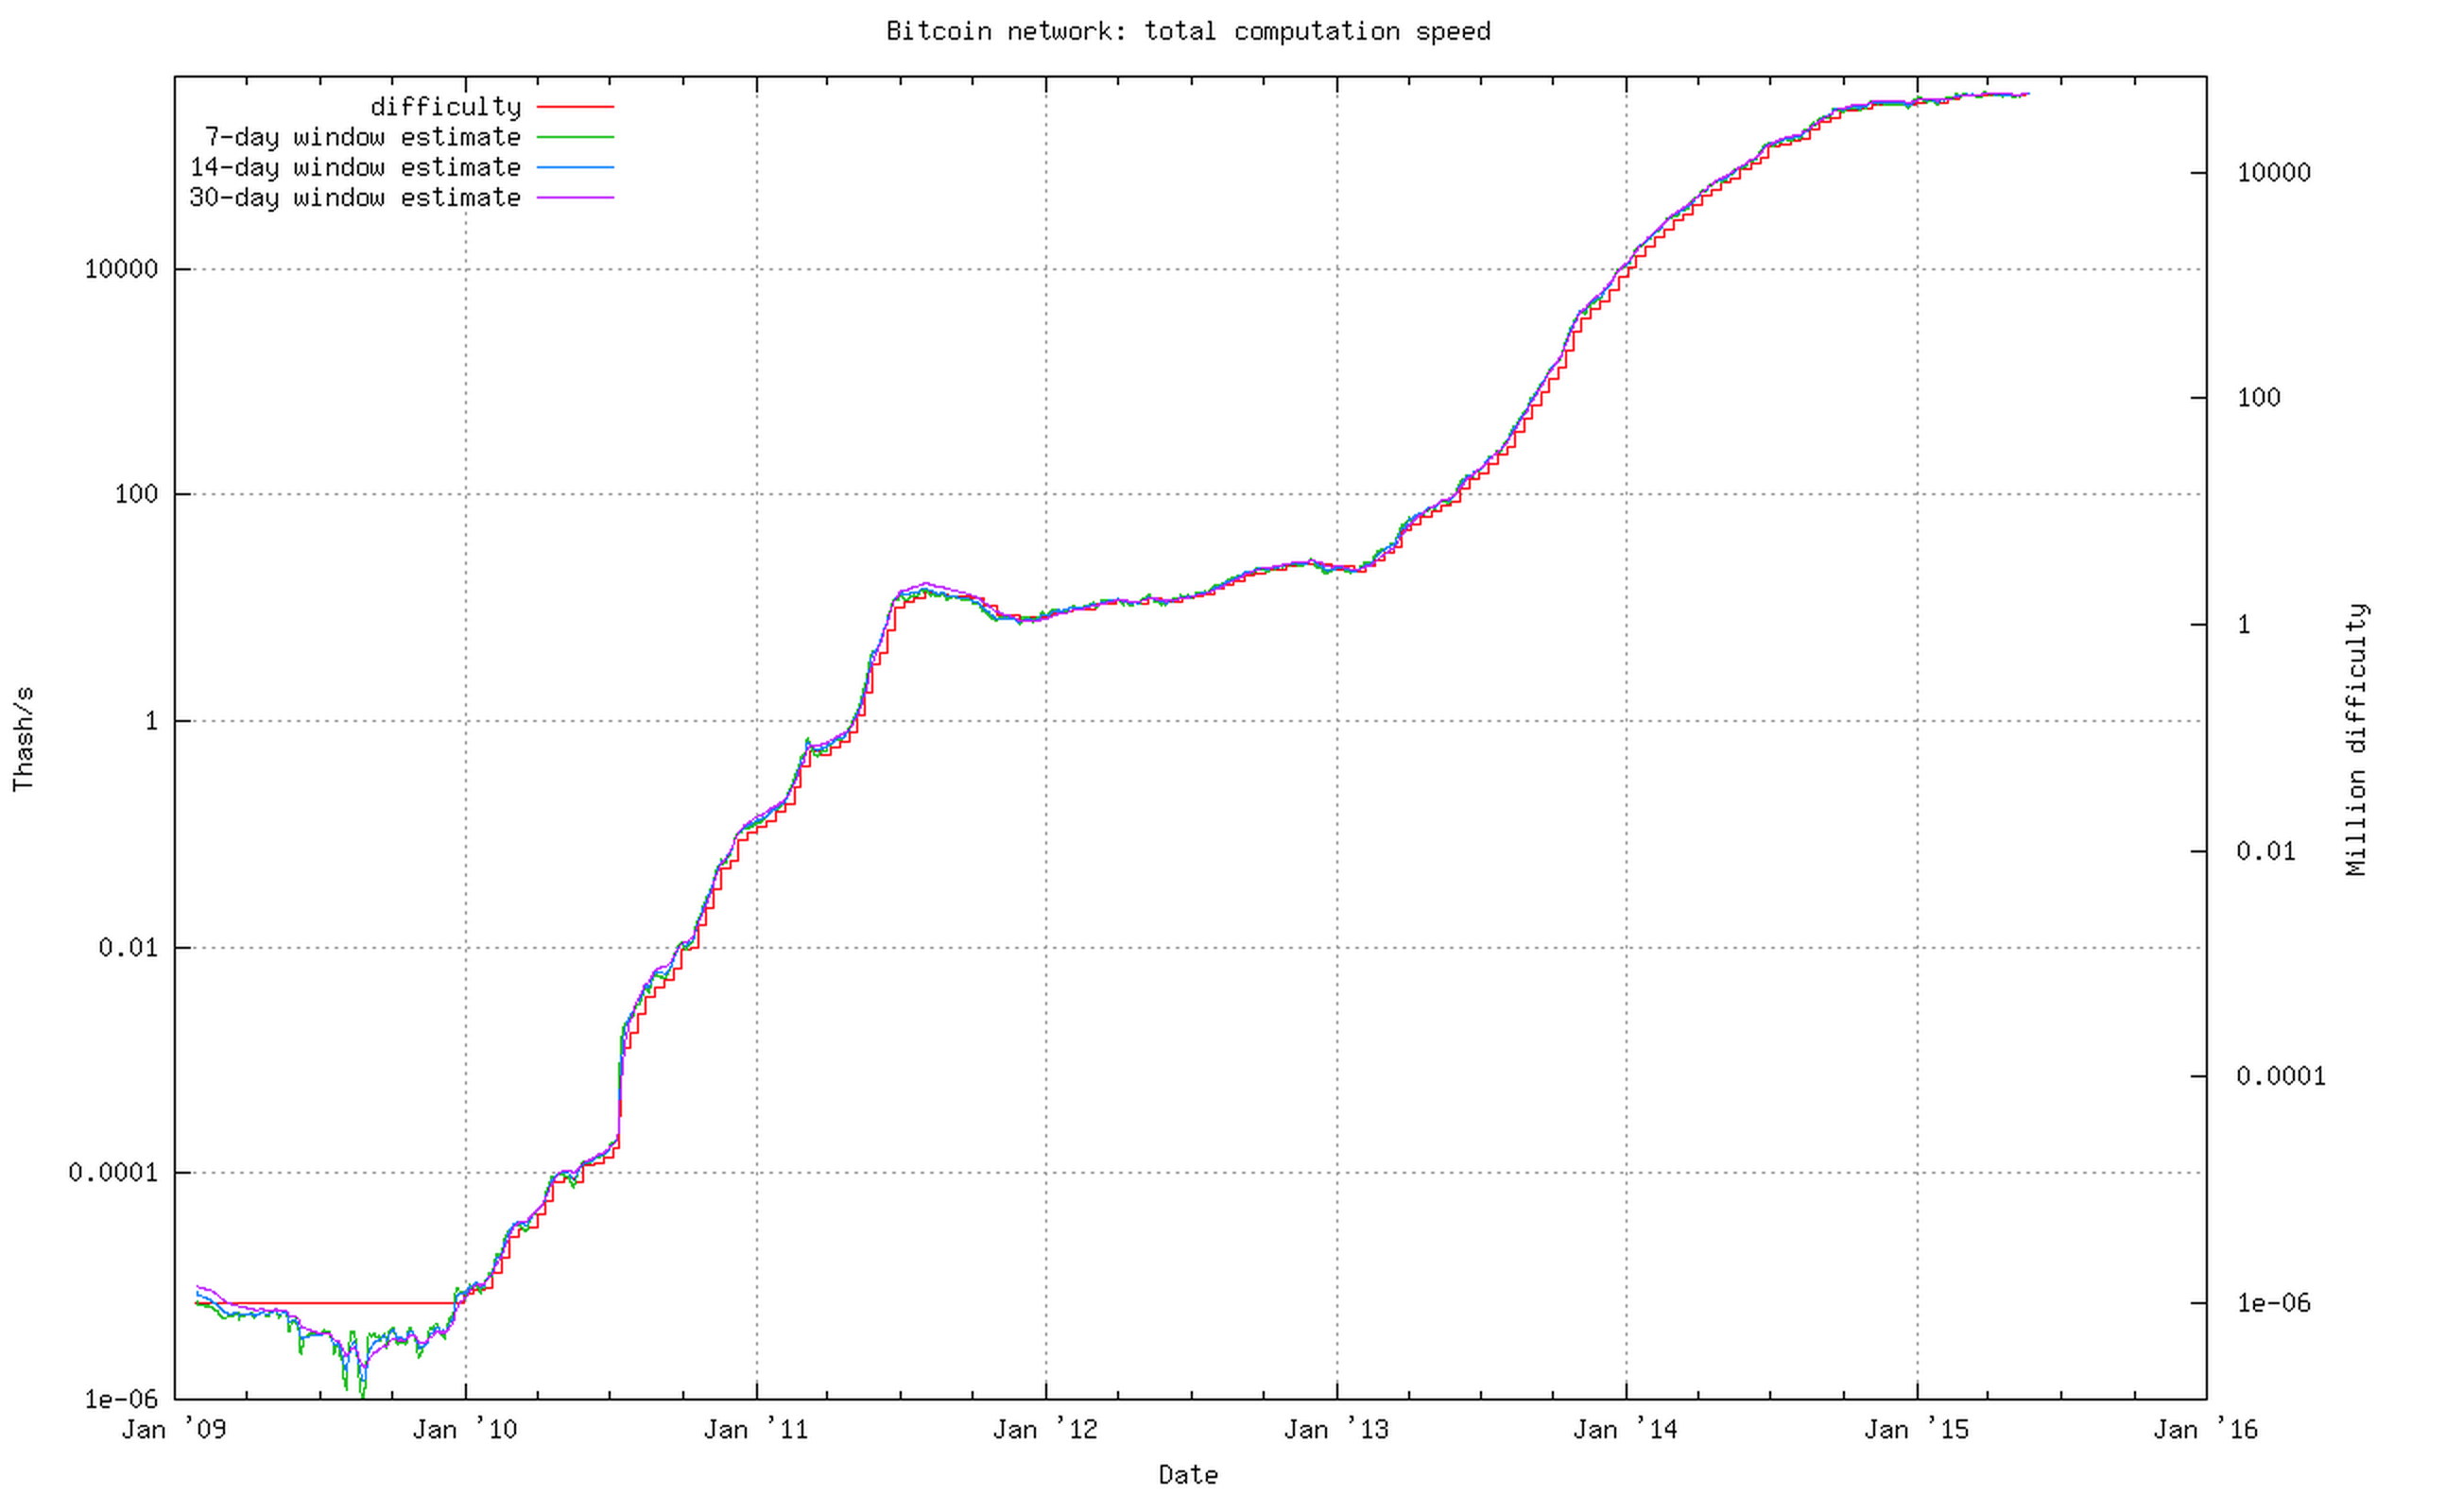
\includegraphics[width=0.95\textwidth]{Figures/Bitcoin/Difficulty-all}
    \caption{The bitcoin mining difficulty, from the beginning until today \cite{bitcoin-charts}.}
    \label{fig:difficulty}
\end{figure}

To overcome this problem, mining pools were invented. A bitcoin mining pool is a service that distributes
work between miners. The work that is distributed has a lower target value than does the bitcoin network
itself, meaning that each participating miner can find valid blocks faster. Although most of the blocks
submitted to a pool does not fulfill the network requirements, sometimes a block fulfills both the
pool's difficulty requirements \emph{as well as} the network requirements; in that case the new block is
submitted to the bitcoin network and all the miners who submitted work towards finding the block
is rewarded according to their contribution.

As such, pooled mining lets anyone with weaker hardware participate in bitcoin mining in exchange for
a smaller reward. However, using hardware such as regular CPUs and GPUs is still considered unprofitable
because of these processors' relative performance compared to specialized bitcoin mining ASICs, as
discussed in section \ref{sec:bitcoin-history}.

\section{The SHA-256 Hash Algorithm}

The SHA-256 hash algorithm is defined in FIPS180-4 \cite{fips180-4} and is a member of the SHA-2
family of hash functions. Like all hash functions, it works by accepting an arbitrary
amount of input data and producing a constant-length output. The function is one-way,
that is, given a hash, it is impossible to determine the input data used to produce
the hash.\todo{Mention all 3 attributes}

The SHA-256 algorithm works on blocks of 512~bits. Each of these blocks are expanded into a
block of 64 32-bit long words using a message expansion function. Each of these words are
used as input to one iteration of the SHA-256 compression algorithm, which uses simple bitwise functions
such as shifts, rotations, logic functions and unsigned addition to create a 256~bit
output value. Each round of the compression function is dependent on the output data from
the previous round in addition to the current input word from the expanded message block
and a constant.

After 64 iterations of the compression function, the result is added to the intermediate
hash values from any previous blocks, or, if there are no previous blocks, the initial
hash value, producing a finished hash.

A more detailed description of the algorithm can be found in appendix \ref{app:hashing-algo}.

In the bitcoin system, a double SHA-256 algorithm is used. To obtain a double hash, the
output of a previous SHA-256 calculation is simply used as input data to the hashing
algorithm. \cite{fips180-4}

% Is this too little or too vague?

\section{Evolution of Bitcoin Mining Hardware}
\label{sec:bitcoin-history}

Because of the bitcoin currency's popularity and the competitiveness involved in mining it, there exists
many different accelerators to improve the performance and energy efficiency of mining systems.
During the currency's history, hardware for bitcoin mining has evolved from regular, general-purpose
CPUs to highly specialized ASIC-based systems.

The bitcoin blockchain was started on January 3rd, 2009. At this point, all mining was done
using CPU mining. The official bitcoin network client supports mining and was used for this
purpose. The fastest CPU miner, a high-end, overclocked Core i7 990x eventually reached 33~MH/s
using SIMD extensions in order to improve performance. \cite{bitcoin-history}

\subsection{GPU Mining}
The shift to GPU mining started in July 2010, when the first OpenCL miner was written and
used in a private mining setup. In September that year, the first open source GPU miner,
which was based on Cuda, was released after the author was paid 10~000 bitcoins, worth about
\$600 USD at the time, by Jeff Garzik, one of the core bitcoin developers. An open source
OpenCL-based miner was released shortly after. \cite{bitcoin-history}

OpenCL miners typically compute the double SHA-256 hash using a fully unrolled implementation
of the compression loop. Multiple hash calculations are run simultaneously exploiting the parallelism
offered by GPUs. Many miners tweaked various parameters of their hardware, such as the voltage and
clock frequencies of both the video RAM and the GPU core in order to get higher throughput
and thus reduce the cost of running each GPU, in order to obtain greater profits \cite{bespoke-silicon}.
% Maybe mention rigs?

\subsection{FPGA Mining}
\label{sec:fpga-mining}

FPGA miners appeared in June 2011, providing better energy efficiency compared to GPUs \cite{bespoke-silicon}.
Early designs were mostly based on the Spartan 6 FPGAs from Xilinx, and could provide a
performance of between 200~MH/s and 220~MH/s per chip, about the same as contemporary GPUs \cite{bitcoin-hardware-cmp},
but consuming as little as a fifth of the power used by their GPU counterparts \cite{bespoke-silicon}.
One example of such an FPGA design is the BTCMiner, an open-source bitcoin miner firmware for
ZTex' FPGA boards, which can obtain up to 215~MH/s with a power usage of about 9,8~W, giving
21~MH/J \cite{btcminer}.

% Note: Taylor managed to get the release year of the GPUs he compares performance to wrong,
% choosing GPUs from 2012 to compare to FPGAs from 2011.

FPGAs provided great advantages to the speed of bitwise functions, which are important for
the SHA-256 algorithm. Popular open-source designs were created so that they could be used
by different kinds of FPGAs. They consisted of a SHA-256 module which had a configurable depth pipeline, each
consisting of the necessary hardware for computing a specific number of rounds of the
SHA-256 compression function. Completely unrolling the algorithm created a pipeline of
64 stages, with a throughput of 1 hash per cycle, but it was also possible to specify
lesser unroll factors which resulted in fewer pipeline stages and reduced throughput, taking
several cycles to perform a hash, but saving registers and logic resources in the FPGAs.
The pipelines were duplicated to improve performance.

Power consumption became much higher than typical for FPGAs, with the pipelined design
giving an extremely high activity factor for LUTs. Development boards could not provice enough
power and heat dissipation for sustained usage, and development of custom boards that focused
on providing enough power and cooling with minimal unused resources, became popular. \cite{bespoke-silicon}

\subsection{ASIC Miners}
\label{sec:asic}

Neither GPUs nor FPGAs can compare to ASICs, specialized chips that started to appear on the network
in the beginning of 2013 \cite{first-asic-miner}. It was the need for more high-performance and power
efficient bitcoin miners caused implementors of bitcoin miners to turn to ASIC solutions.

One of the first ASIC designs were Butterfly Labs' ASIC miners. Having experience developing
FPGA based mining solutions, the company created an ASIC chip with 16 double SHA256 modules,
the equivalent of 16 FPGA-based miners using a 65~nm process. The end-product ended up being
delayed when the chips ended up consuming more power than expected and had to be underclocked
in order to be able to cool the chips properly.

ASICMINER was another of the earliest designs, including only one SHA256 hash unit on a chip,
replicating a single FPGA-based design at a much higher frequency, with better energy efficiency
and a cheaper price. \cite{bespoke-silicon}

\subsubsection{The Goldstrike 1}
Another ASIC design is the Goldstrike 1 architecture, noteworthy because its architecture is
described in an article in IEEE Micro by Javed Barkatullah and Timo Hanke \cite{goldstrike}.
Because of the competitive nature of bitcoin mining, it is not common for designers of ASIC
solutions to reveal too many details about the architecture of their chips and few scientific
papers exist on the topic.

The Goldstrike is an ASIC-based bitcoin mining solution capable of reaching 2~TH/s. To reach the performance
requirements, a bitcoin mining core was created that was able to perform at 125 GH/s. Four of
these were combined in one package, with four of these packages then combined on a circuit board
to produce the target performance.

The Goldstrike cores consist of an architecture with 120 hash engines running in parallel.
A hash engine searches through all possible values of the 32-bit nonce field in the bitcoin header
(see section \ref{sec:bitcoin-mining}) in order to find a valid hash.

The hash engines uses a pipelined double-SHA-256 implementation, with each round of the hash calculation
unrolled into a pipeline.

The finished ASIC chips, each with four bitcoin mining cores, were measured to provide 504~GH/s while using
500~W of power. This gives an energy efficiency of about 1~GH/J.

Interestingly, the architecture provided challenges with regards to to powering and cooling the chips.
Because the architecture uses all available computing power for bitcoin mining all the time while
the chips are in use, no parts of the chips can be turned off to save power. \cite{goldstrike}

% Fun fact, GH/Ws = GH/J

%\subsection{Scaling of bitcoin hardware}
%Due to the dark silicon problem, future chips will require that parts be powered down or deactivated
%in order to satisfy a given power budget \cite{dark-silicon2}. Bitcoin mining may be close to
%the worst case for dark silicon optimizations, far beyond multicore CPUs or GPUs. Due to bitcoin
%mining's high processing requirements, the logic needed to run the algorithm cannot be turned off without losing
%performance.
%
%Butterfly Labs ran into this problem with their 65~nm chip, and had to scale back the performance to reduce power consumtion
%and manage to cool the chip properly. While bitcoin mining began as a ``race to ASIC'', energy costs now determine
%which ASICs are the most profitable and therefore energy efficiency is a problem that must be addressed. \cite{bespoke-silicon}
%
%Figure \ref{fig:bitcoin-difficulty-devices}, as seen in \cite{bespoke-silicon}, shows the same up to 2014, but also hightligts when each generation was released, from CPU to ASIC.
%
%\textbf{Comment the development. Find facts about it. (currently lower priority)}

%\begin{figure}[htb]
%    \centering
%    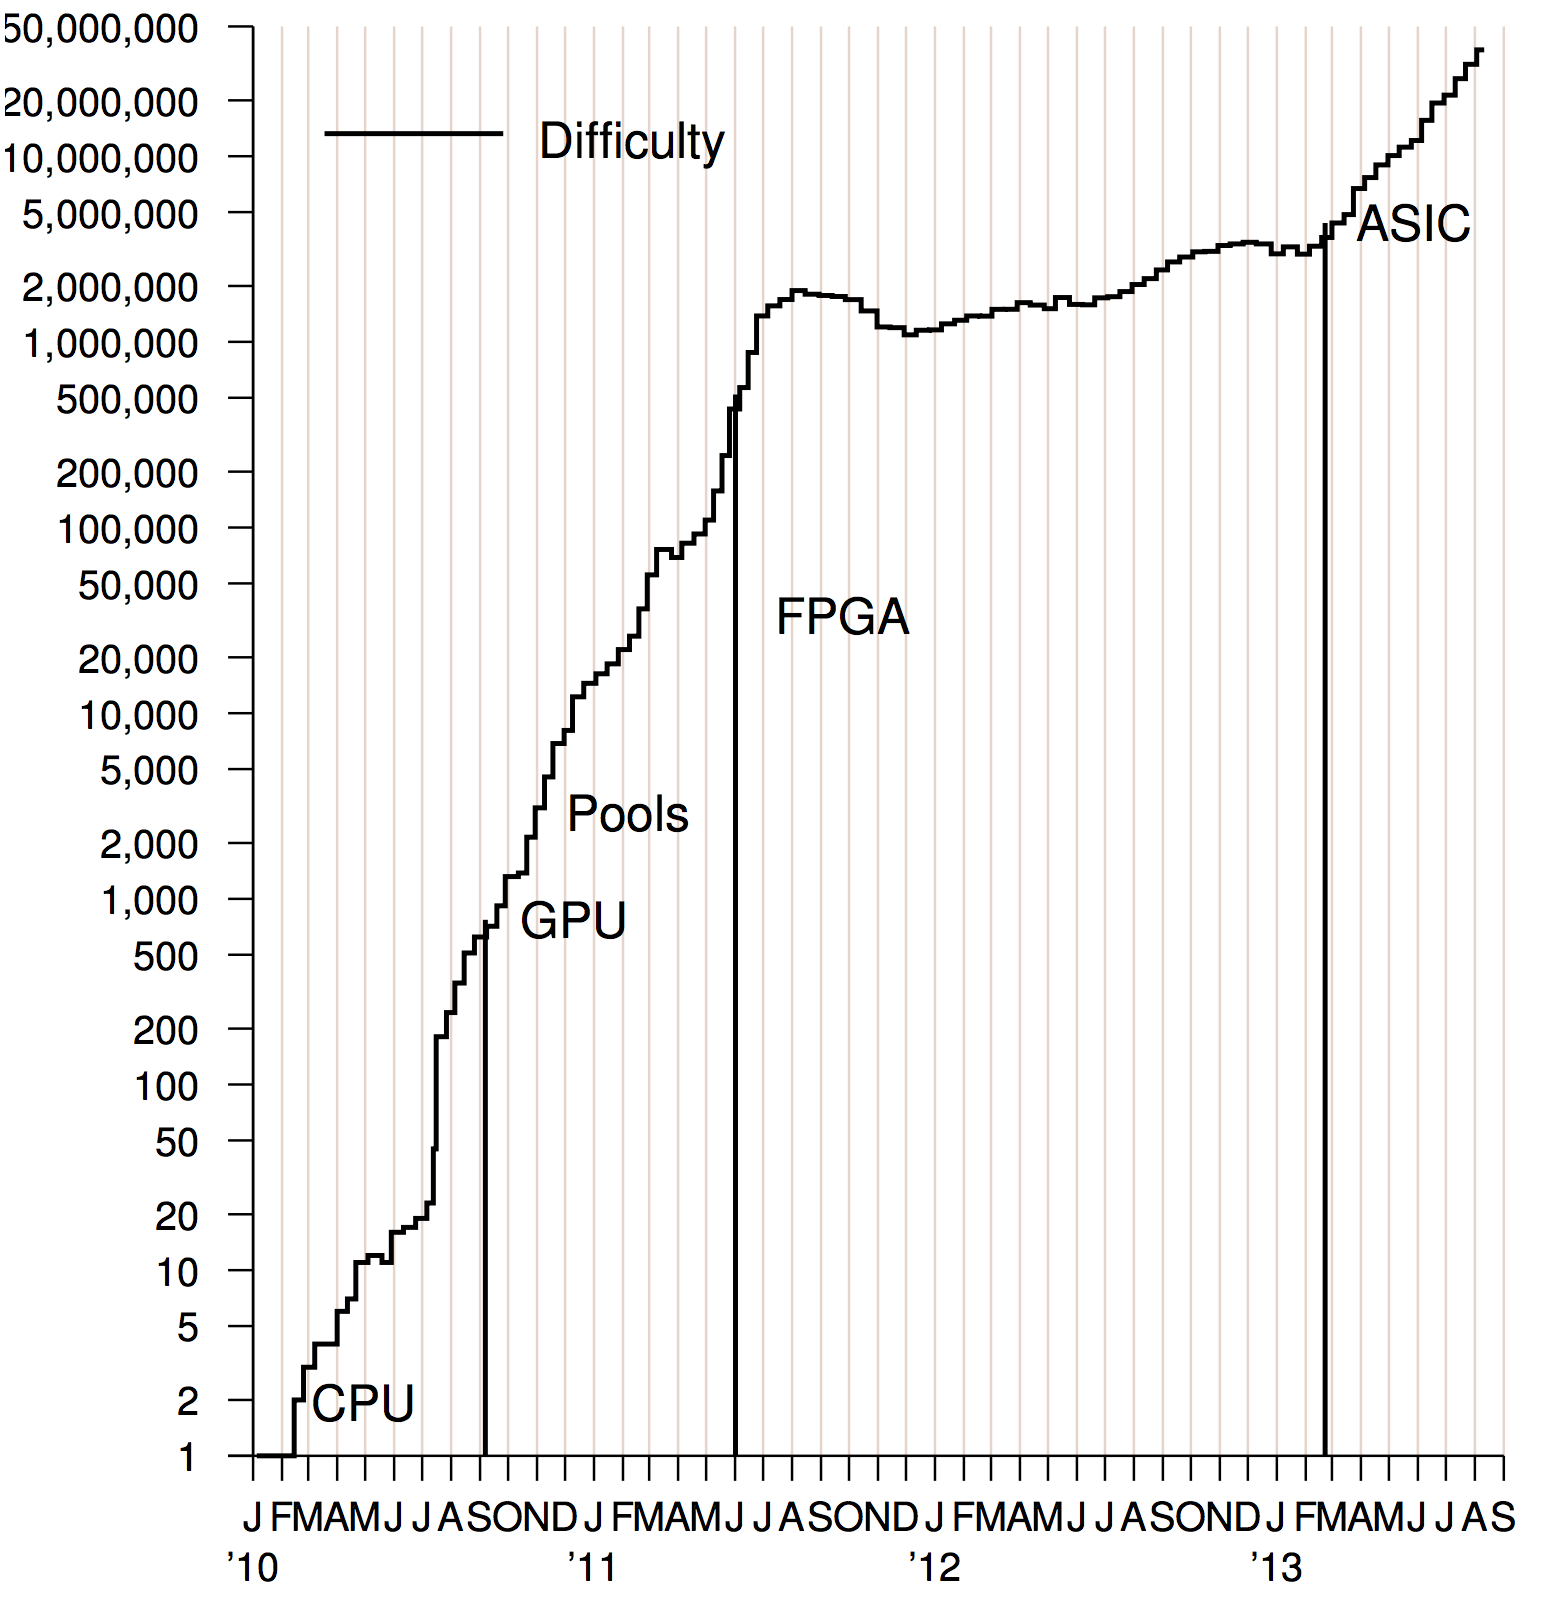
\includegraphics[width=0.95\textwidth]{Figures/Bitcoin/Difficulty-devices}
%    \caption{The BTC Mining Difficulty, compared to when each generation was introduced, as seen in \cite{bespoke-silicon}.}
%    \label{fig:bitcoin-difficulty-devices}
%\end{figure}

\section{The Problem of Dark Silicon}
\label{sec:dark-silicon}

Moore's law states that transistor density on integrated chips will continue to double every
two years. This has turned out to match reality pretty well, and in addition, native transistor speeds are increasing with a factor of 1,4.
According to the principle of Dennard scaling, which predicts that the power density of transistors, that
is the voltage and current used to operate the transistor, would scale down with the
size of the transistors, this would not be a problem; however, the energy efficiency
of transistors is only improving by a factor of 1.4.

Under a constant power-budget, there is a shortfall of a factor of 2 in the energy budget,
and this utilization potential of a chip is falling exponentially by 2 times for each generation.
If the power limitation were to be based on the current generation, then designs would be 93,75\% dark in eight years.
This gives rise to the term ``dark silicon'', where a chip must either be underclocked or parts of
it turned off in order to stay within a defined power budget, giving rise to ``dark'' areas of the chip.
This is especially true for chips where the cooling solutions are no longer efficient enough to remove
the generated heat from a fully powered chip.

In an attempt to work around this problem, the CPU industry moved to using multicore processors around 2005.
Since the gains from improving instruction level parallelism were diminishing, the industry focused more on thread level parallelism and throughput through multiprocessing \cite{computer-architecture}.
However, adding multiple cores does not circumvent the problem in the long run.
Multicore chips will not scale as transistors shrink, and the fraction of a chip that can be filled with cores running at full frequency is dropping exponentially with each processor generation. 
Large fractions of the chip will be left dark --- either switched off for a long time, or significantly underclocked. \cite{dark-silicon}
%New designs are required, with new architectural techniques that spend area to buy energy efficiency. \cite{dark-silicon}

\subsection{Approaches to the Problem of Dark Silicon}
\label{sec:taylor}

To work around the problem of dark silicon, several approaches have been suggested.
In \cite{dark-silicon}, Taylor have listed up three particular approaches: shrinking the chips, dimming the chips, and specializing the chips.
In addition, there is always the possibility that future technology will be a ``deus ex machina'' and solve the problem in
an unexpected fashion.

\subsubsection{Shrinking the Chips}

Instead of having dark silicon on the chip, one can simply shrink the chip itself.
All chips may be shrunk to a certain small extent, but the only chips that truly can gain from shrinking only, will be those on which dark silicon is only a waste, and cannot be used to further enhance the product.   
Specalizing into these types of shrunk chips may, however, turn out to be less profitable business, as further generations of Moore's law adds little benefit. 

Futhermore, there are other disadvantages: exponentially smaller chips are not necessarily exponentially cheaper, since mask cost, design cost and I/O pad aread does not also become cheaper. 
%Competition will most likely favor chips that utilizes dark silicon to improve the overall product, thus chips that are only shrinked will sell at low market price, leading to loss for the company.
Exponential shrinking also leads to exponential rise in power density, and chip temperature will rise.
Meeting the temperature limit will increase the cost, at which the scaling of energy efficiency is reduced below the nominal 1.4 factor.
%Meeting the temperature limit will reduce the scaling below the expected energy effeciency, at the nominal \todo{Feels weird}1.4X scaling.

\subsubsection{Dimming the Chips}
The term ``dim silicon'' refers to the use of general purpose logic that typically employs heavy underclocking or infrequent use.
As such, large amounts of otherwise dark silicon area is put to productive use while meeting the power budget.
While the fraction of dark transistors on chips increases exponentially, the silicon area becomes exponentially cheaper
as a resource, relative to the power and energy consumption. This gives the opportunity to spend area to buy energy efficiency.
Dark silicon areas can be populated with logic that is used only part of the time.

Lately, more elegant methods are emerging. Among the dim silicon techniques are dynamically varying the frequency with the
number of cores being used, scaling up the amount of cache logic, employing near threshold voltage (NTV) designs, and redesigning
architectures to accommodate bursts that temporarily allow the power budget to be exceeded, such as Intel's Turbo Boost technology. \cite{dark-silicon}

\subsubsection{Specialization}
Instead of using general purpose logic, this approach focuses on specialized use of logic for selected tasks.
Within a set of processors, each are specialized for a subset of tasks, increasing energy efficiency or performance compared to a general purpose processor, for those particular tasks.
An application is executed on the processor which is deemed the most efficient for the task.
Cores not in use are power and clock gated so as to not waste energy unnecessarily.

%Specialized accelerators are heavily used today, especially in fields such as media and graphics and mobile phone processors.
%These enable orders-of-magnitude improvements in energy efficiency and performance for certain types of computations.
%Systems with more coprocessors than general purpose processors, referred to as coprocessor-dominated architectures, or CoDAs, is predicted to become more and more common.

Challenges with these systems are expected as well, one of them being the so-called ``Tower of Babel'' crisis, where
the notion of general-purpose computation becomes fragmented, and the clear lines of communication between programmers and software and the underlying hardware is no more.
There are several cases of overspecialization problems between accelerators, where many of them cannot be used for closely related classes of computation.
For instance, CUDA for NVidia GPUs cannot be used for similar architectures, such as AMD GPUs.
Specialized hardware also risk becomming obsolete when standards are revised. \cite{dark-silicon}

\subsubsection{Deus Ex Machina}
The term ``deus ex machina'' comes from literature and theater, in which the protagonists seem increasingly doomed until the very last moment, when something completely unexpected comes out of nowhere to save the day.
In the case of dark silicon, a deus ex machina would be a major breakthrough in semiconductor device technology.
The required breakthrough would have to be very fundamental, making it possible to build circuits out of devices other than MOSFETs. 
There are physical limits to what can be done with for instance leakage from MOFSET transistors, and transistors made of other materials may go beyond these limits.
New transistors must also be able to compete with MOFSETs in performance.
Tunnel field-effect transistors (TFET) and nanoelectromechanical system switches (NEMS) are examples of inventions that may hint to order-of-magnitude improvements to the leakage problem, although they still fall short in performance. \cite{dark-silicon}

\subsection{Benefits of Heterogeneous Architectures}
\label{sec:heterogeneous}

Specialized heterogenenous architectures offers various possibilities for improved performance and energy efficiency;
this could be in the system's ability to adapt to various applications or even external conditions such as
power or temperature conditions \cite{heterogeneous-ee, heterogeneous-perf, heterogeneous-arch}.
This has been explored in \cite{heterogeneous-ee}, \cite{heterogeneous-perf} and \cite{heterogeneous-arch}.
By combining different processors from the Alpha Family, Kumar \textit{et al} has proven that heterogenous architecture does excel in energy efficiency and performance, compared to a homogeneous system.
In a simluation the EV4 (Alpha 21064), EV5 (Alpha 21164), EV6 (Alpha 21264) and a single-threaded version of EV8 (Alpha 21464) were combined into a heterogeneous multi-processor.
The SPEC2000 benchmark were run with one application on one core at a time, with the others powered down.
The simulation showed that 32~\% of the energy were saved with performance loss of only 2.6~\% relative to the EV8 core, when using best static scheduling, and using dynamic core switching with simple heuristics further improved the results. \cite{heterogeneous-ee}

In another simulation where system performance were the main goal, a combination of EV5 and EV6 onto a 100 mm$^2$ chip were simulated, where the size of EV6 equals the size of four EV5.
The tradeoff was between greater single-threaded performance of the more complex EV6 versus greater thread-level parallelism of adding more EV5 cores.
The best homogeneous designs could fit either four EV6 cores or 20 EV5 cores on the chip, and for the simulation, three EV6 and five EV5 were chosen to form a heterogeneous multi-core processor.
Instead of one single application, the simulation tested the best global assignments when running multiple threads, from a small number of the SPEC2000 benchmarks.
Threads that exploited the EV6 better would be given assigned to the more complex cores.
Compared to a homogeneous multi-prosessor system with four EV6, the simulation showed that the heterogeneous system performed up to 37~\% better with an average 26 \% improvement over the configuration, considering 1-20 threads.
Compared to 20 EV5 cores, the performance was up to 2.3 times better, and averaged 23~\% better over that same range.
Using dynamic heuristics for core assignment further increased the performance.
\todo{Sentence a bit vague. See if it can be improved, or delete it.}Additionally, the heterogeneous system was tested for its tolerance against increasing job queues, and a homogeneous system with four EV6 becoma saturated much earlier than the heterogeneous system, showing that the latter has higher tolerance to larger amount of work, given the increased thread-level parallelism.
\cite{heterogeneous-perf}
%\begin{figure}[htb]
%    \centering
%    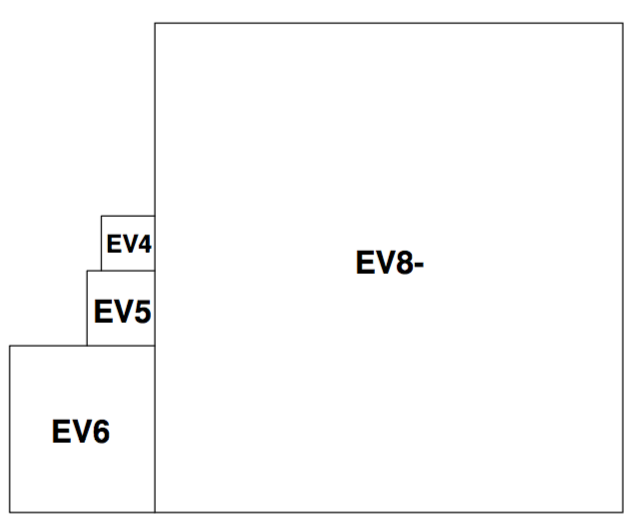
\includegraphics[width=0.5\textwidth]{Figures/Heterogeneous/Kumar1}
%    \caption{Cores used in \cite{heterogeneous-ee}, and their relative sizes.}
%    \label{fig:Kumar1}
%\end{figure}


%\begin{figure}[htb]
%    \centering
%    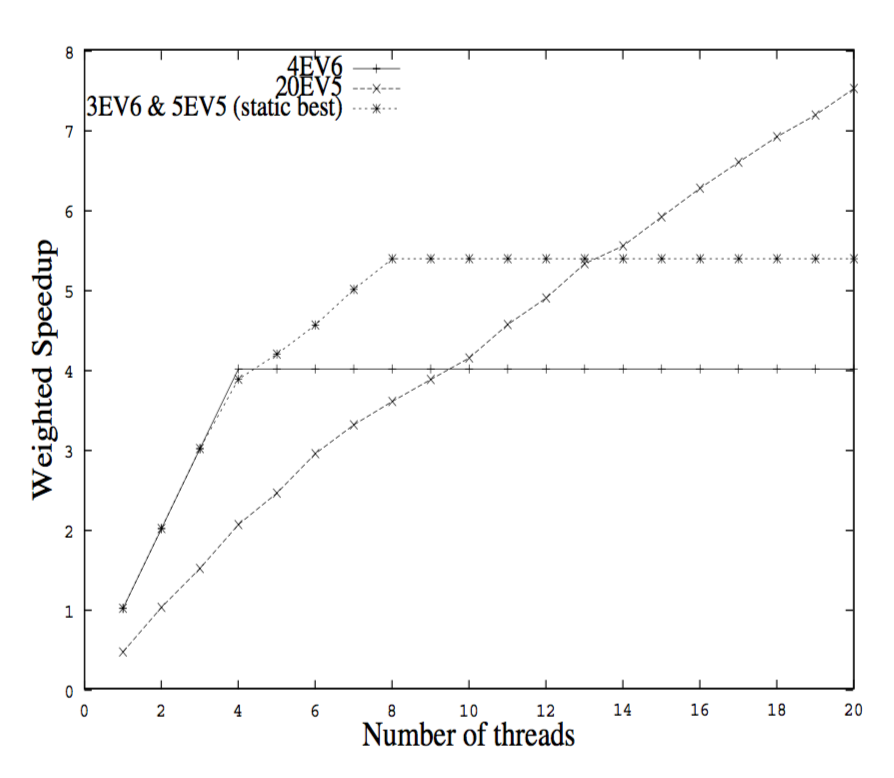
\includegraphics[width=0.5\textwidth]{Figures/Heterogeneous/Kumar2}
%    \caption{Weighted speedup, relative to EV6, when comparing the heterogenous multiprocessor with best homogeneous multiprocessors using EV5 and EV6 \cite{heterogeneous-perf}}
% %**NOTE: The figure text makes no sense!
% Better now?
%    \label{fig:Kumar2}
%\end{figure}

%In addition to testing the performance gain, Kumar \textit{et al} also tested the the response time within the job queue as well.
%This was to give insight on how well heterogeneous processors handles large job queues, compared to the best homogeneous systems.
%For this test, jobs with an average distribution of 200 million cycles were generated randomly and executed.
%Then different mean job arrival rates with exponential distribution were simulated.
%It was revealed a great difference between saturation for a homogenous system with 4 EV6 processors and the heterogeneous processor.
%For the former, the unbounded response time was seen as the arrival rate approached its maximum throughput around 2 jobs per 100 million cycles.
%From there, the run queue became infinite. % %**NOTE: This makes no sense!
%Beyond this point, due to the saturation, the response time became infinate. %Better now?
%The heterogeneous system remained stable well beyond that point.
%The degradation was also more graceful under heavier loads than for homogeneous processors.
%This can be seen in figure \ref{fig:Kumar3}.

%\begin{figure}[htb]
%    \centering
%    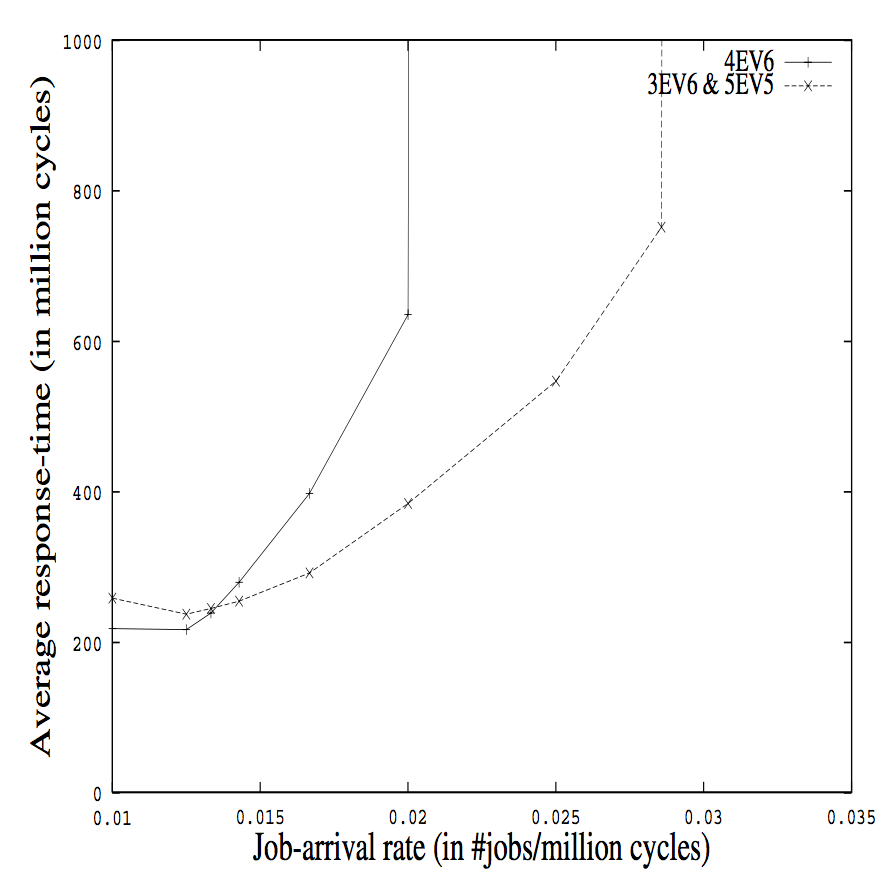
\includegraphics[width=0.5\textwidth]{Figures/Heterogeneous/Kumar3}
%    \caption{Limiting response-time for various loads \cite{heterogeneous-perf}.}
%    \label{fig:Kumar3}
%\end{figure}

\cite{heterogeneous-arch} takes a closer look at what can be considered a good heterogeneous design, in making the heterogeneous multiprocessor from scratch instead of using pre-existing core designs.
Using pre-existing cores presents lower flexibility in choices, while best heterogeneous designs are composed of specialized core architectures.
The study in \cite{heterogeneous-arch} came to the following conclusions:
\begin{itemize}
\item The most efficient heterogeneous multiprocessors were not constructed from cores that make good general-purpose uniprocessor cores, nor cores that would appear in good homogeneous multicure architectures.
\item Each core should be individually tuned for a class of applications with common characteristics.
%      This usually results in non-monotonic processors.
\item And performance advantages of heterogeneous multiprocessors also hold for completely homogeneous workloads (where the task has no differences).
    In those cases, the diversity across different workloads are exploited.
\end{itemize}

The more constrained the area or power budget, the more benefit the heterogeneous designs provide, as homogeneous systems were able to run to the fullest on generous budgets only.
As future designs become more aggressive, with more cores added to the chip, the results underline the impact heterogeneous design will have for the future. 

\section{The Single-ISA Heterogeneous MAny-core Computer}
\label{sec:shmac}

The Single-ISA Heterogeneous MAny-core Computer is an architecture designed for investigating heterogeneous
systems at all abstraction levels, as illustrated in figure \ref{fig:shmacAbstractionLevels}.
It implements a tile-based architecture with a mesh interconnect. All processor tiles implement the same
ARM ISA and the same memory model, in order to achieve a common programming model \cite{shmac-plan}.
A high-level illustration of SHMAC can be seen in figure \ref{fig:shmac}.

Because the programming model is kep constant, the underlying implementation of the system can change.
This means that the same application can be run on SHMAC instances with different tile layouts or on
SHMAC instances implemented on different physical media, such as in FPGAs or ASICs. Currently, SHMAC
is only run on FPGAs.

\begin{figure}[htb]
    \centering
    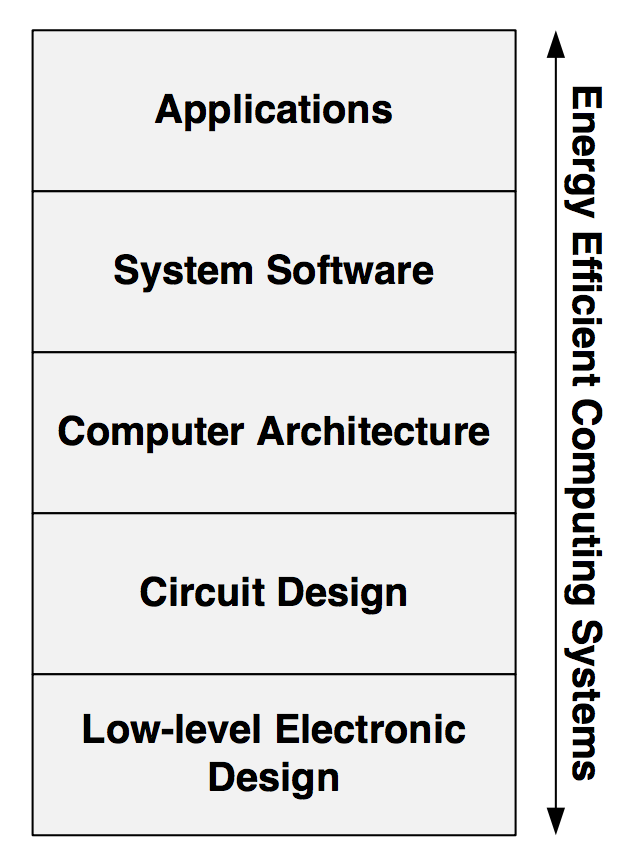
\includegraphics[width=0.5\textwidth]{Figures/Heterogeneous/SHMACAbstractionLevels}
    \caption{Levels of abstraction in computing systems \cite{shmac-plan}.}
    \label{fig:shmacAbstractionLevels}
\end{figure}

\begin{figure}[htb]
    \centering
    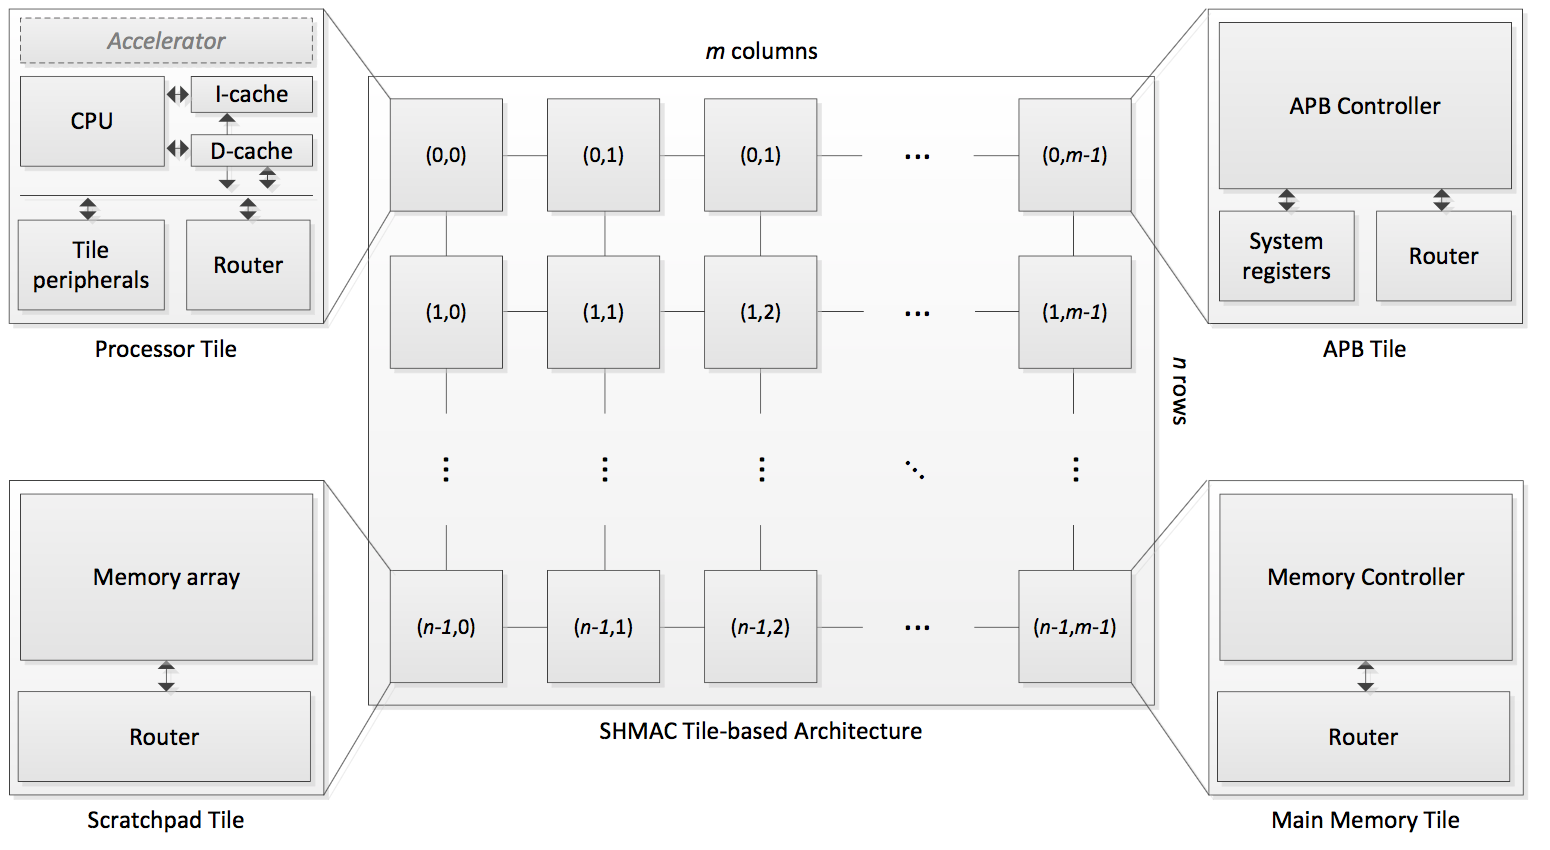
\includegraphics[width=0.95\textwidth]{Figures/Heterogeneous/SHMAC}
    \caption{High-Level architecture of SHMAC \cite{shmac-plan}.}
    \label{fig:shmac}
\end{figure}

\subsection{Versatile Express}

\textbf{Write specs here. Explain the FPGA}

\subsection{SHMAC Architecture}

SHMAC is a tile-based architecture, with the processing elements laid out in a rectangular
grid with neighbour-to-neighbour connections, using a mesh interconnect with XY-routing.
%Several tile types are currently supported, not including the tile described in this report,
%with the most important ones being the processor tile, which contains a Turbo Amber CPU
%\footnote{See section \ref{sec:aht} for a short overview}, a scratchpad tile which functions as
%fast temporary storage, a DRAM tile and an I/O tile for communicating with a host system.

Several tile types are supported. The main ones are:

\begin{description}
    % Torbjørn: Joined Amber and Turbo Amber.
  \item[Processor Tile] Currently two versions are supported: the open source ARM Amber CPU, and an improved version called Turbo Amber.
  	The original Amber core provides support for the ARMv2a instruction set, while the Turbo Amber
	provides support for the ARMv4t instruction set, giving the core the ability to also execute
	instructions from the 16-bit Thumb instruction set. Several performance optimizations are
	also added to the core \cite{turboamber}. An overview of the processor tile can be seen in
	figure \ref{fig:shmac-cpu}.
  \item[Scratchpad Tile] --- A memory tile providing a small amount of memory for use by software.
  	This memory is provided by the on-chip block RAM resources of the FPGA \cite{shmac-plan}.
  \item[DDR Memory Tile] --- Memory controller tile that gives SHMAC access to off-chip DDR memory.
  \item[APB Interface (I/O tile)] --- This tile implements the Advanced Peripherals Bus (APB) slave
  	which gives the host processor on the Versatile Express board access to SHMACs memory space
	for use when programming the memories \cite{shmac-plan}.
  \item[Dummy Tile] --- Empty tile which only contains router functionality \cite{shmac-plan}. Can be used for instance
  	as a filler tile.
\end{description}

\begin{figure}[htb]
    \centering
    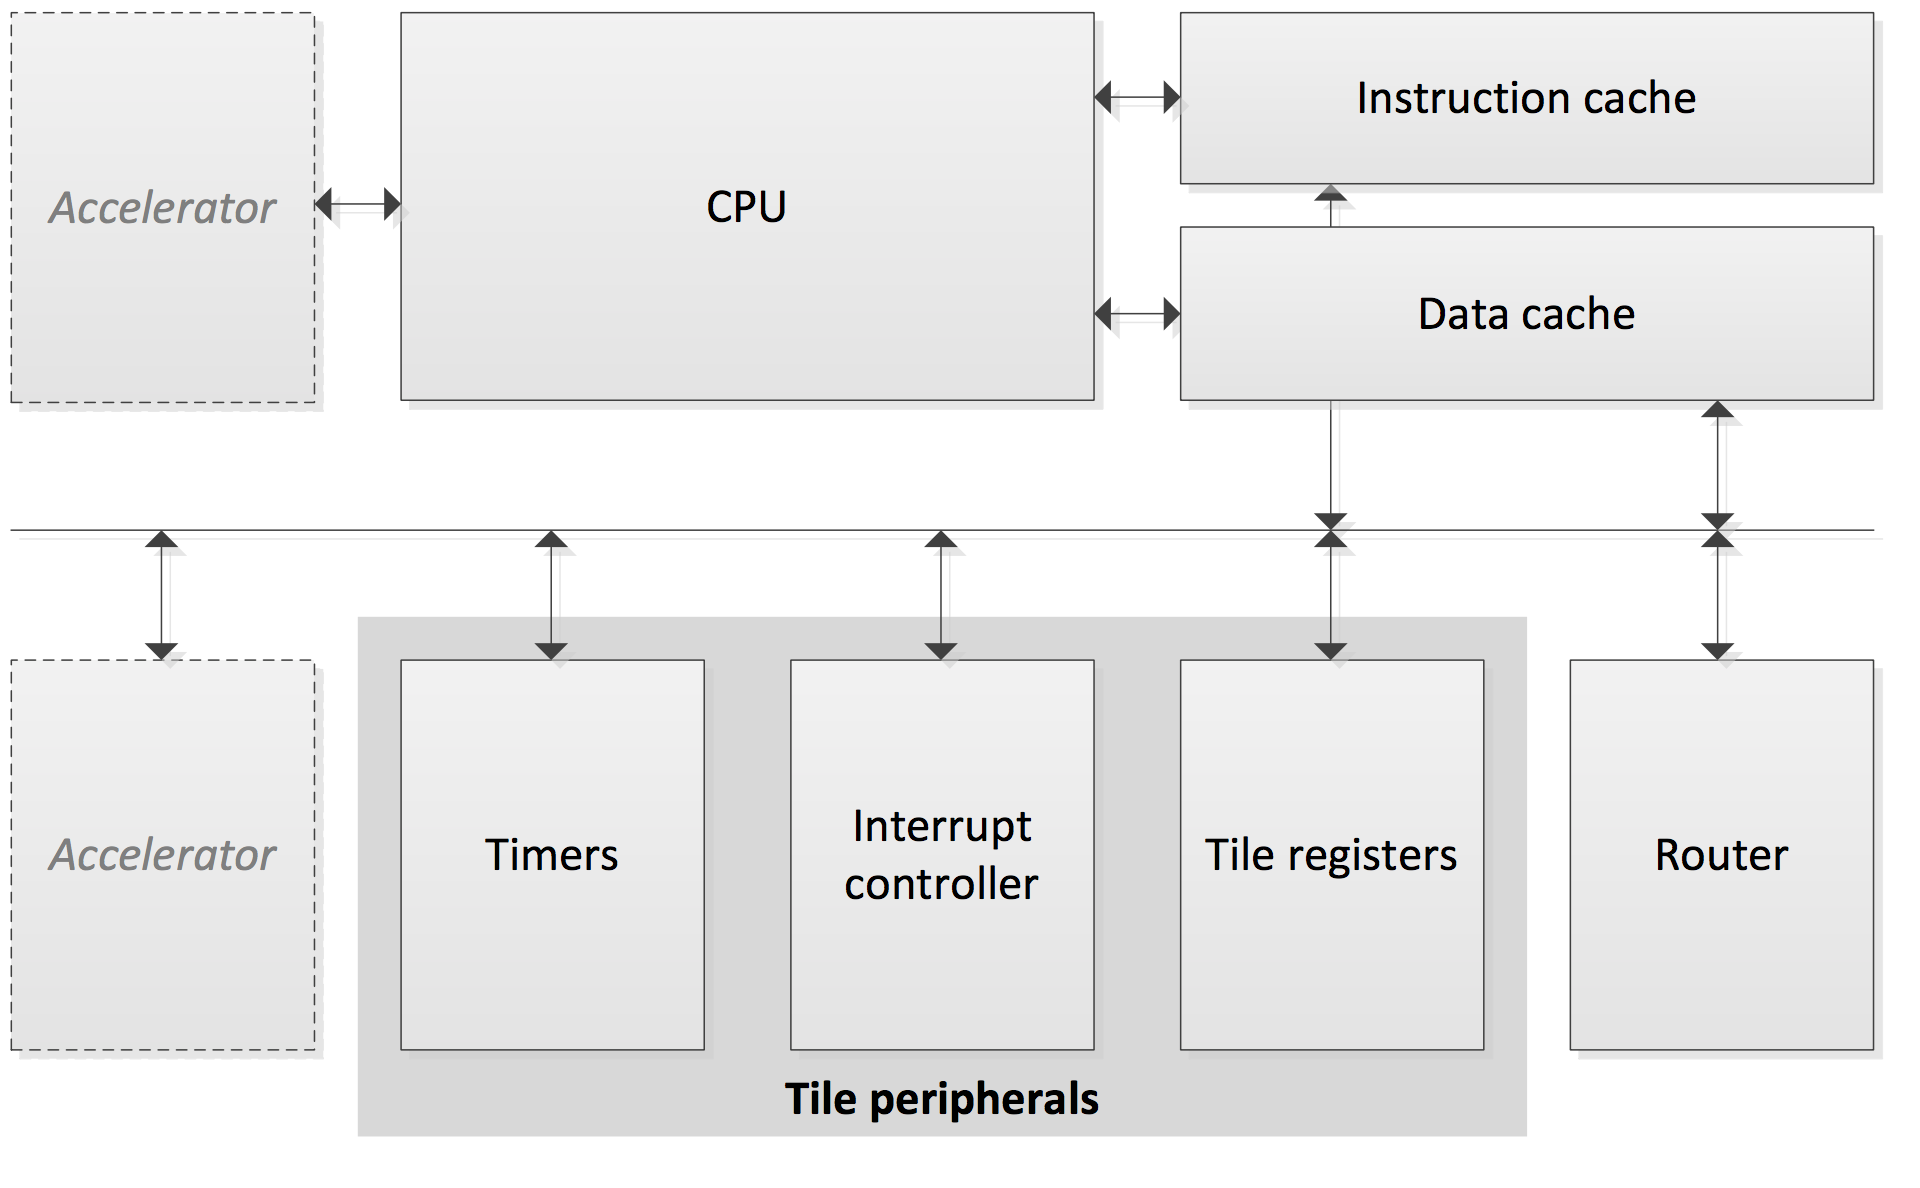
\includegraphics[width=0.8\textwidth]{Figures/Heterogeneous/SHMACCPU}
    \caption{SHMAC processor tile \cite{shmac-plan}.}
    \label{fig:shmac-cpu}
\end{figure}

\subsection{SHMAC Memory Map}
% *** NOTE: I seriously don't think this is relevant information, suggest removing this section.
% Torbjørn: Disagree, it affects our software programming, when using SHA-256 module, DMA module and Scratchpad memory. Everything that affects our project should be mentioned.

Figure \ref{fig:shmac-memory} shows how the memory is mapped in the ARM-based SHMAC. All
processor tiles share the same address space with only the tile register space being
private for each tile. This memory area contains information about the tile itself, such as its coordinates,
the CPU ID number and other useful data. In addition the tile register space contains the memory-mapped
peripherals for each tile, such as timers and the interrupt controller.
Any custom peripheral, such as the DMA and the hashing accelerator developed in the project is mapped into this address space.
The system registers are used for communication with the host system.

\begin{figure}[htb]
    \centering
    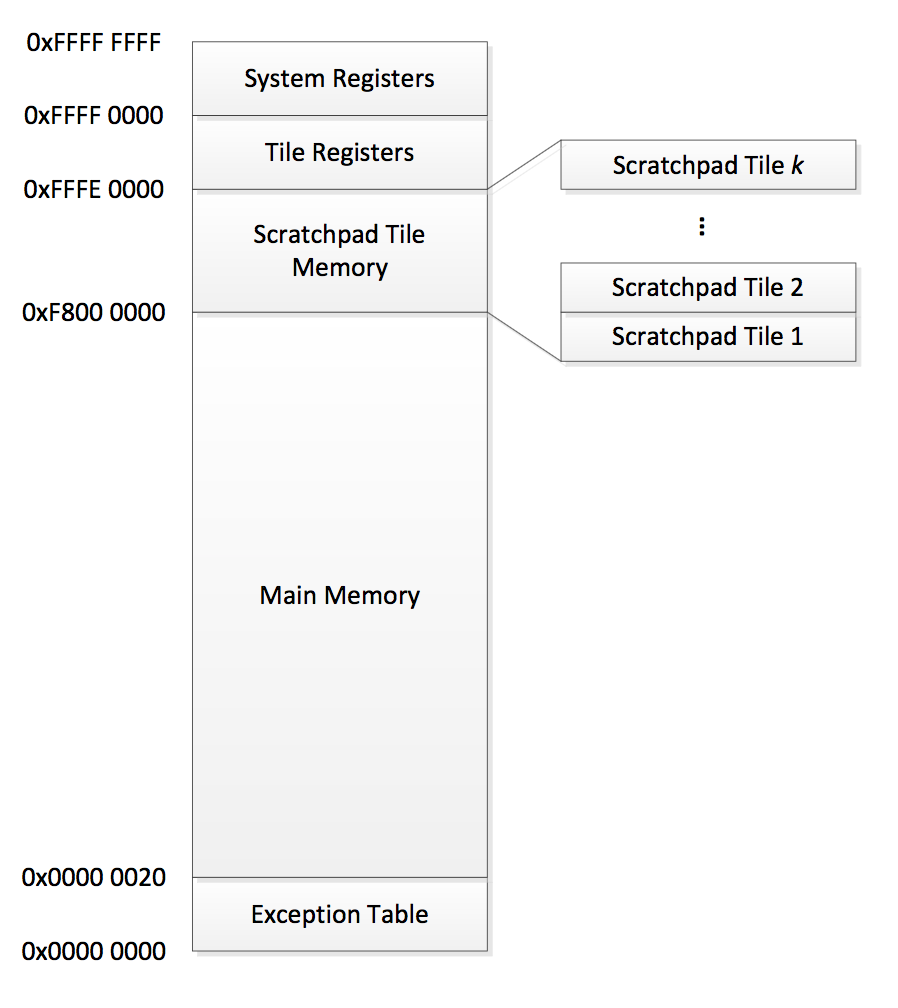
\includegraphics[width=0.6\textwidth]{Figures/Heterogeneous/SHMACMemory}
    \caption{Memory map of ARM-based SHMAC, as seen in \cite{shmac-plan}.}
    \label{fig:shmac-memory}
\end{figure}

\subsection{SHMAC Interconnection Network}

SHMAC utilizes a 2D mesh-based interconnection network to connect all the tiles, which is used to transport data packets of 128~bits length.
Store-and-forward switching with on/off flow control is used, and the XY-algorithm is used for deciding the route of each data packet.
Each tile consists of a router with five ports, one for each of its neighbours and the local connection.
When multiple packets are inbound from different directions, a round-robin scheme is used to arbitrate between which
packet to route through, and packets from the local tile has equal priority to those arriving from the other directions. \cite{shmac-plan}

In the current implementation, it takes 3 cycles for a data packet to transfer from one tile to the next. 
The architecture of the router can be seen in figure \ref{fig:shmac-router}.

\begin{figure}[htb]
    \centering
    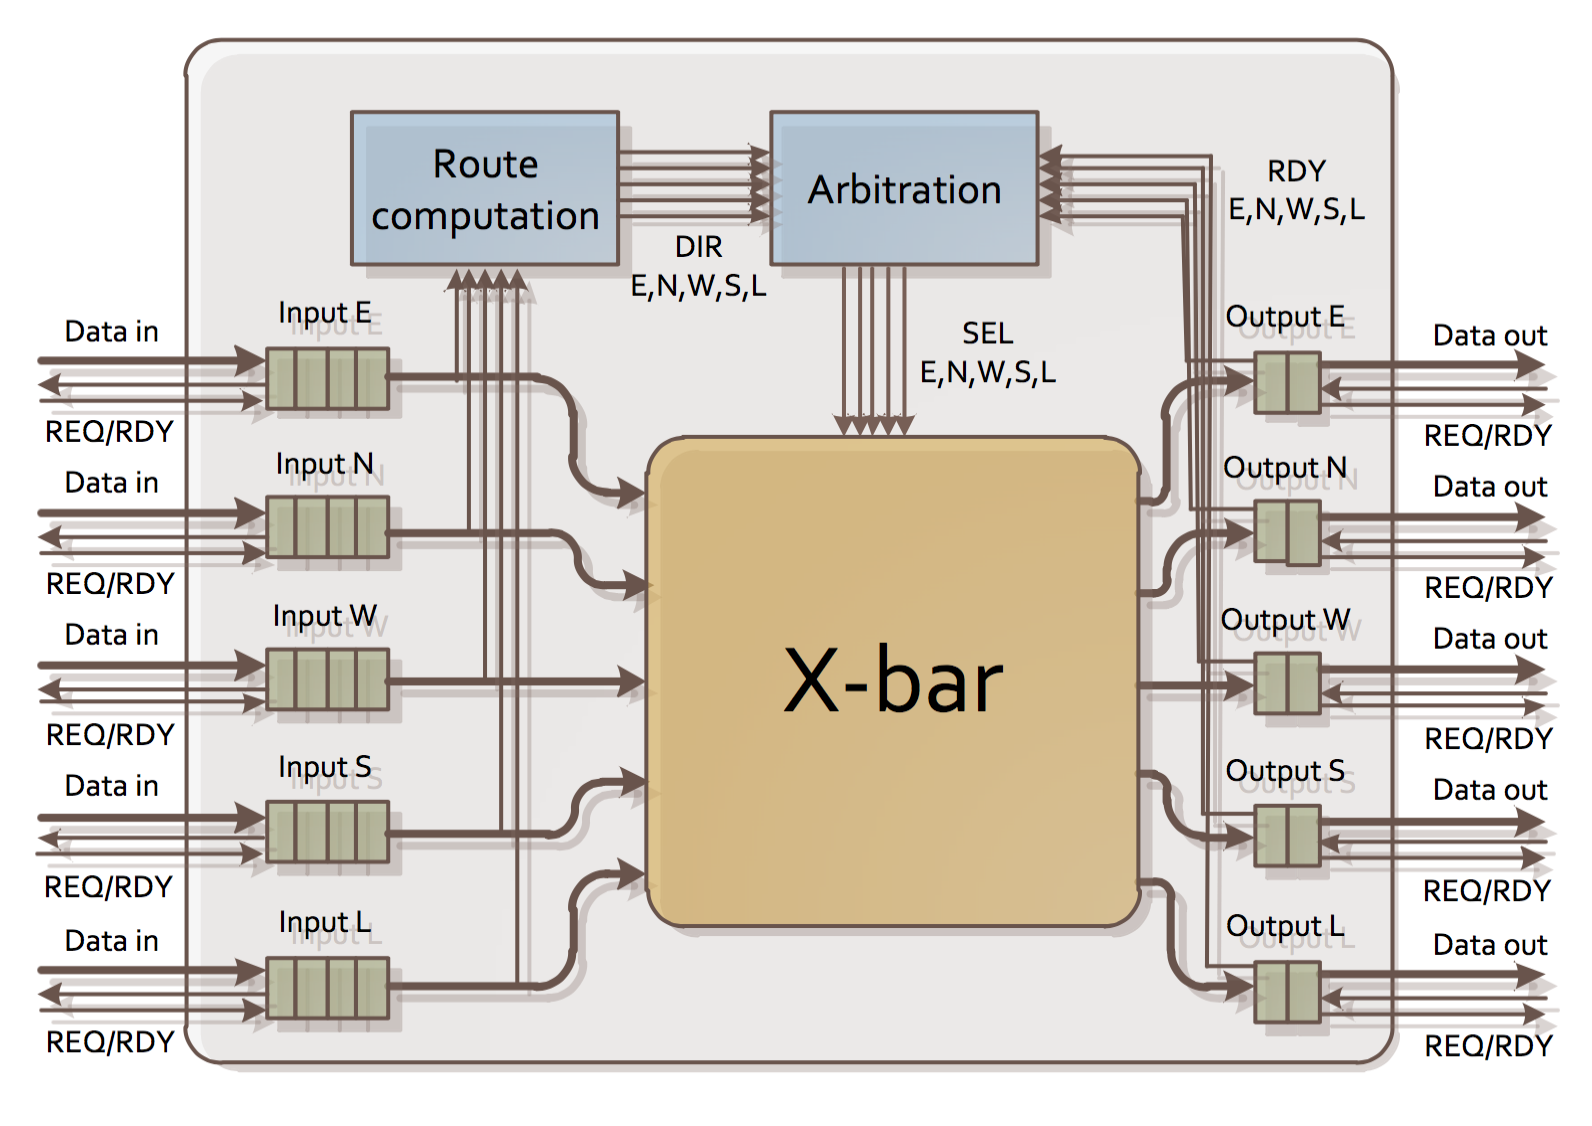
\includegraphics[width=1.0\textwidth]{Figures/Heterogeneous/SHMACRouter}
    \caption{Architecture of the SHMAC router \cite{shmac-plan}.}
    \label{fig:shmac-router}
\end{figure}

\subsection{Wishbone Bus}

Wishbone is a bus architecture developed by OpenCores to create a common interface for use between IP cores, especially in
open source designs. It supports single-word transfers as well as burst transfers. A pipelined transfer mode is also provided
which allows multiple requests to be sent from a module without the module having to wait for an acknowledge.

Wishbone is used as internal bus on the CPU tiles of SHMAC. Burst or pipelined transfers are
not currently supported, neither internally on the tiles, or by the interconnect network, which can limit performance.

\section{Greater throughput using DMA Module}

\textbf{Describe WHY DMA, briefly}

%WISHBONE is implemented as internal bus on the CPU tiles of SHMAC, but currently supports only single transfers with no bursts or pipelining.
%This means that in spite of using switched packet interconnection network on SHMAC, something that opens up for sending out several packets, a WB Master on a tile will only send out one request, before getting the acknowledged response back.
%\todo{Yaman said this. Find out if oral conversations with teachers/staff is allowed for bibliography.}\cite{Yaman}
%And prior to this project, only one WB master existed on each tile, owning the entire WISHBONE network in the tile.
%
% % ***NOTE: Actually, the mesh interconnect does not support burst transfers as far as I understood. It is hard not to support Wishbone burst transfers... and almost no one uses pipelined transfers in Wishbone.
%  Torbjørn: So, we just mention it. Easy-peasy
